\documentclass[tikz,border=6pt]{standalone}
\usepackage{pgfplots}
% If your TeX is older, use 1.17 instead of 1.18
\pgfplotsset{compat=1.17}
\usetikzlibrary{arrows.meta}

\begin{document}
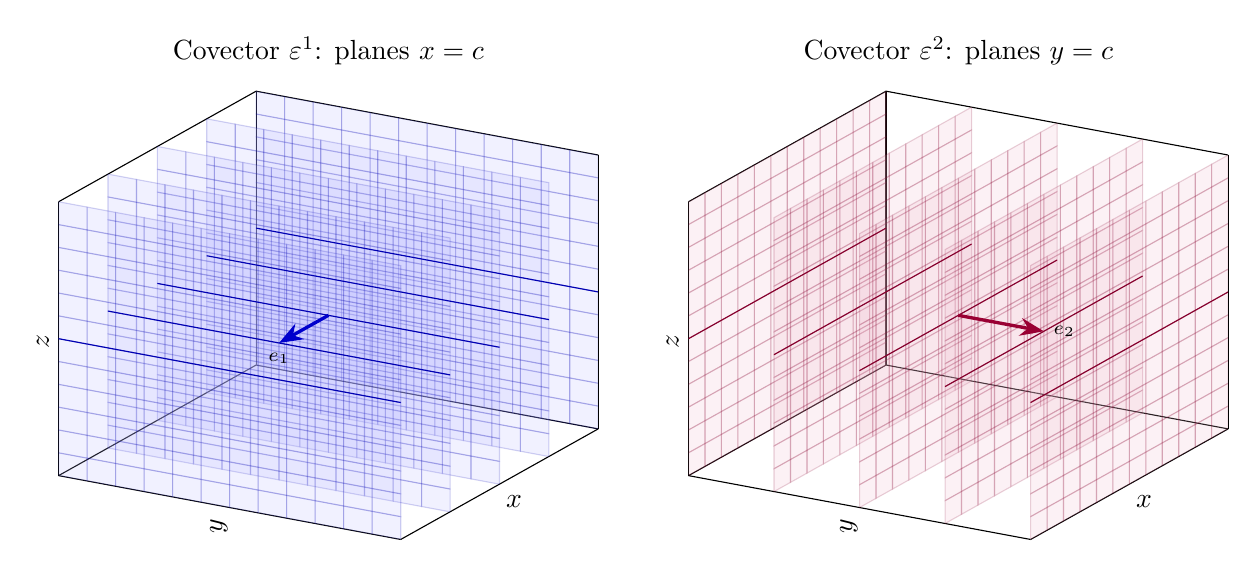
\begin{tikzpicture}	
	% ============ Left axis: epsilon^1 (planes x = c) ============
	\begin{axis}[
		name=left,
		title={Covector $\varepsilon^1$: planes $x=c$},
		view={120}{25},
		axis lines=box, ticks=none,
		xmin=-2, xmax=2, ymin=-2, ymax=2, zmin=-2, zmax=2,
		xlabel={$x$}, ylabel={$y$}, zlabel={$z$},
		]
		% A few planes x = c (literal constants)
		\addplot3[surf, opacity=0.18, draw=blue!70!black, fill=blue!30,
		shader=flat corner, domain=-2:2, y domain=-2:2, samples=13, samples y=13]
		({-2}, x, y);
		\addplot3[surf, opacity=0.18, draw=blue!70!black, fill=blue!30,
		shader=flat corner, domain=-2:2, y domain=-2:2, samples=13, samples y=13]
		({-1}, x, y);
		\addplot3[surf, opacity=0.18, draw=blue!70!black, fill=blue!30,
		shader=flat corner, domain=-2:2, y domain=-2:2, samples=13, samples y=13]
		({0},  x, y);
		\addplot3[surf, opacity=0.18, draw=blue!70!black, fill=blue!30,
		shader=flat corner, domain=-2:2, y domain=-2:2, samples=13, samples y=13]
		({1},  x, y);
		\addplot3[surf, opacity=0.18, draw=blue!70!black, fill=blue!30,
		shader=flat corner, domain=-2:2, y domain=-2:2, samples=13, samples y=13]
		({2},  x, y);
		
		% little trace on z=0 to show where the plane slices the xy-plane
		\addplot3[blue!70!black] coordinates {(-2,-2,0) (-2,2,0)};
		\addplot3[blue!70!black] coordinates {(-1,-2,0) (-1,2,0)};
		\addplot3[blue!70!black] coordinates {( 0,-2,0) ( 0,2,0)};
		\addplot3[blue!70!black] coordinates {( 1,-2,0) ( 1,2,0)};
		\addplot3[blue!70!black] coordinates {( 2,-2,0) ( 2,2,0)};
		
		% e1 axis arrow (normal to planes x=c)
		\addplot3[-{Stealth[length=3mm]}, very thick, blue!80!black]
		coordinates {(0,0,0) (1,0,0)};
		\node at (axis cs:1,0,0) [below, font=\scriptsize] {$e_1$};
		
%		% sample point and vector (all literals)
%		\addplot3[only marks, mark=*, mark size=1pt]
%		coordinates {(0.3,-0.4,0.6)};
%		\addplot3[-{Stealth[length=2.4mm]}, very thick, orange!80!black]
%		coordinates {(0.3,-0.4,0.6) (1.2,-0.7,1.0)};
	\end{axis}
	
	% ============ Right axis: epsilon^2 (planes y = c) ============
	\begin{axis}[
		xshift=8cm,
		title={Covector $\varepsilon^2$: planes $y=c$},
		view={120}{25},
		axis lines=box, ticks=none,
		xmin=-2, xmax=2, ymin=-2, ymax=2, zmin=-2, zmax=2,
		xlabel={$x$}, ylabel={$y$}, zlabel={$z$},
		]
		% planes y = c (literal constants)
		\addplot3[surf, opacity=0.18, draw=purple!70!black, fill=purple!30,
		shader=flat corner, domain=-2:2, y domain=-2:2, samples=13, samples y=13]
		(x, {-2}, y);
		\addplot3[surf, opacity=0.18, draw=purple!70!black, fill=purple!30,
		shader=flat corner, domain=-2:2, y domain=-2:2, samples=13, samples y=13]
		(x, {-1}, y);
		\addplot3[surf, opacity=0.18, draw=purple!70!black, fill=purple!30,
		shader=flat corner, domain=-2:2, y domain=-2:2, samples=13, samples y=13]
		(x, {0},  y);
		\addplot3[surf, opacity=0.18, draw=purple!70!black, fill=purple!30,
		shader=flat corner, domain=-2:2, y domain=-2:2, samples=13, samples y=13]
		(x, {1},  y);
		\addplot3[surf, opacity=0.18, draw=purple!70!black, fill=purple!30,
		shader=flat corner, domain=-2:2, y domain=-2:2, samples=13, samples y=13]
		(x, {2},  y);
		
		% traces on z=0
		\addplot3[purple!70!black] coordinates {(-2,-2,0) ( 2,-2,0)};
		\addplot3[purple!70!black] coordinates {(-2,-1,0) ( 2,-1,0)};
		\addplot3[purple!70!black] coordinates {(-2, 0,0) ( 2, 0,0)};
		\addplot3[purple!70!black] coordinates {(-2, 1,0) ( 2, 1,0)};
		\addplot3[purple!70!black] coordinates {(-2, 2,0) ( 2, 2,0)};
		
		% e2 axis arrow (normal to planes y=c)
		\addplot3[-{Stealth[length=3mm]}, very thick, purple!80!black]
		coordinates {(0,0,0) (0,1,0)};
		\node at (axis cs:0,1,0) [right, font=\scriptsize] {$e_2$};
		
%		% same sample point and vector (literals)
%		\addplot3[only marks, mark=*, mark size=1pt]
%		coordinates {(0.3,-0.4,0.6)};
%		\addplot3[-{Stealth[length=2.4mm]}, very thick, orange!80!black]
%		coordinates {(0.3,-0.4,0.6) (1.2,-0.7,1.0)};
	\end{axis}
\end{tikzpicture}
\end{document}
